\begin{appendices}

\chapter{Project Breathe's patient demographics, treatments and measures list} \label{sec:appendixbreathe}
The figures \ref{fig:breathestats}, \ref{fig:enrolmenttime}, \ref{fig:nintr}, were drawn for study patients enrolled from Royal Papworth and Cardiff Hospitals on the period from 30.12.2019 to 15.06.2021)

\begin{figure}[!htb]
   \begin{minipage}{0.48\textwidth}
     \caption{Patients demographics}
    \centering
    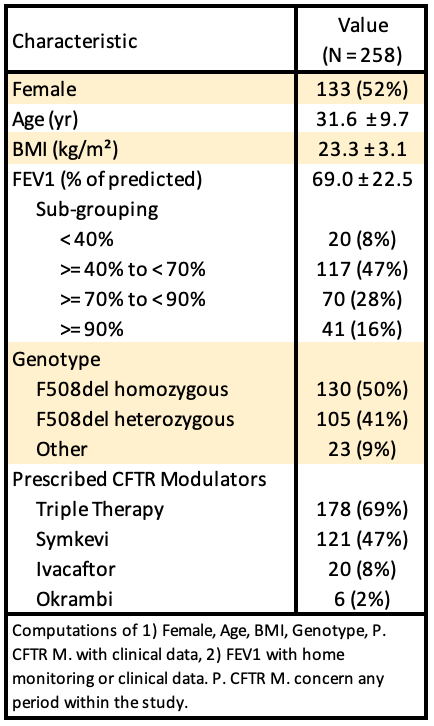
\includegraphics[width=60mm]{images/breathestats.png}
    \label{fig:breathestats}
   \end{minipage}\hfill
   \begin{minipage}{0.48\textwidth}
   
     \caption{Participants' enrolment time}
    \centering
    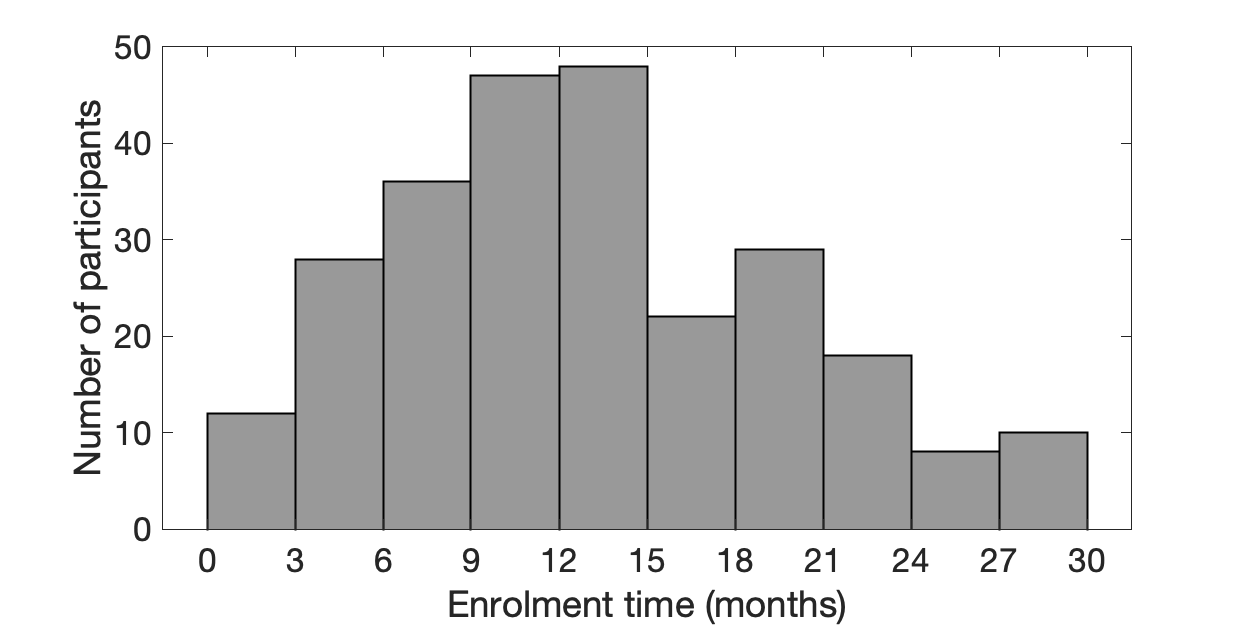
\includegraphics[width=80mm]{images/Patient_enrolment_time_from30-Dec-2019_to15-Jun-2021.png}
    \label{fig:enrolmenttime}
    
    \caption{Number of interventions per participants}
    \centering
    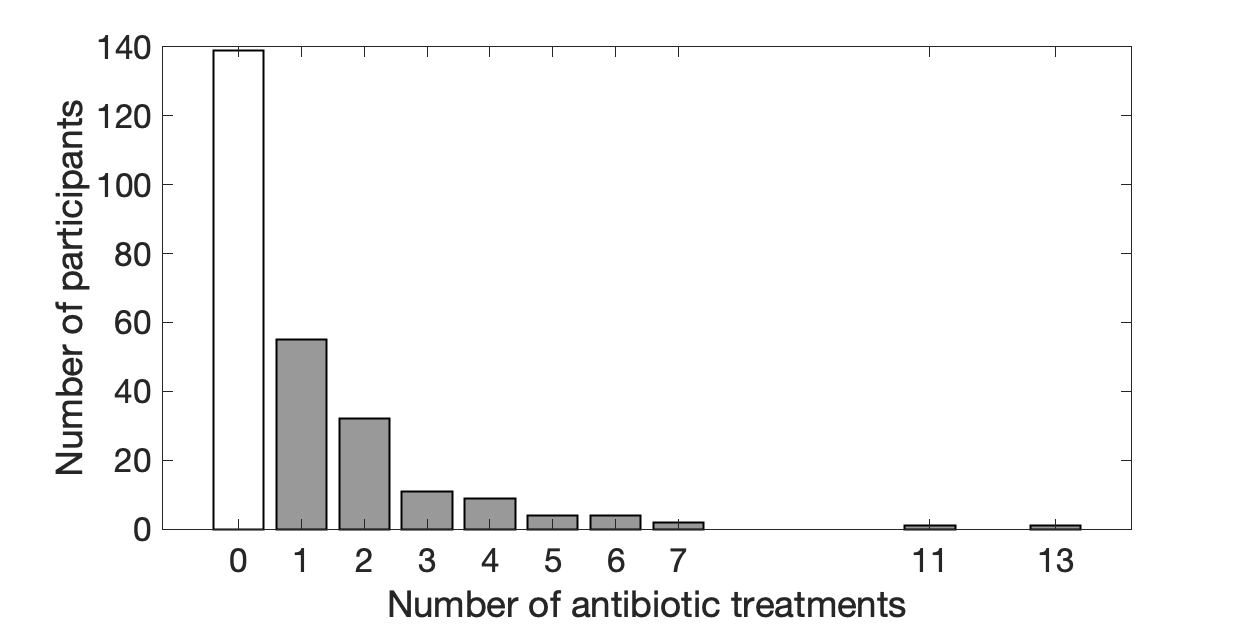
\includegraphics[width=80mm]{images/bar_intrperpatient_before_filter.png}
    \label{fig:nintr}
    
   \end{minipage}
\end{figure}

    
    \begin{table}[]
        \centering
        \begin{tabular}{c|c}
        \hline
             \textbf{CFTR modulator history} & \textbf{Number of participants} \\
             \hline
             Triple Therapy & 85 \\
             Symkevi - Triple Therapy & 78 \\
             No therapy & 35 \\
             Symkevi & 28 \\
             Ivacaftor & 16 \\
             Ivacaftor - Triple Therapy & 3 \\
             Orkambi - Triple Therapy & 3 \\
             Triple Therapy - Symkevi & 3 \\
             Triple Therapy - Therapy stopped & 2 \\
             Ivacaftor - Symkevi & 1 \\
             Symkevi - Triple Therapy - Symkevi & 1 \\
             \hline
        \end{tabular}
        \caption{Participants' CFTR modulators therapy history status on 15.06.2021, chronologically from left to right. }
        \label{tab:cftrmodulators}
    \end{table}

\begin{table}
\begin{tabular}{l|l|l} 

\hline

\textbf{Measure} & \textbf{Description}  & \textbf{Recording method}  \\ 
\hline
Wellness & Answering "How are you feeling today?" & 
\begin{tabular}[c]{@{}l@{}} 1 (Very Unwell) \\ to 10 (Great) \end{tabular}   \\
Cough & Answering 'How is your cough today?"  & 
\begin{tabular}[c]{@{}l@{}} 1 (No Cough) \\ to 10 (Chronic) \end{tabular}   
  \\
FEF2575 & 
\begin{tabular}[c]{@{}l@{}}Mean forced expiratory flow between the 25\% \\and the 75\% of the total volume exhaled\end{tabular}   
\\
FEV075         & Forced expiratory volume in 0.75"   & Spirometer \\
FEV1DivFEV6    & Division of FEV1 by FEV6  & Spirometer\\
FEV1           & Forced expiratory volume in 1"  & Spirometer \\
FEV6           & Forced expiratory volume in 6"  & Spirometer \\
PulseRate      & Heart rate recorded & HR sensor  \\
RestingHR      & Resting heart rate  & Fitbit/AppleHealth \\
O2Saturation   & O2 saturation level & Oximeter \\
Temperature    & Temperature in °C & Themometer   \\
Weight         & Weight in kg & Scale   \\
Calorie        & Calories  & Fitbit/AppleHealth \\
MinsAsleep     & Mintues spent "awake" while sleeping   & Fitbit/AppleHealth \\
MinsAwake      & Minutes spent actually sleeping  & Fitbit/AppleHealth \\
HasColdOrFlu   & Reacting to "I've got a cold or flu" & True/False slider \\
HasHayFever    & Reacting to "I've got hay fever" & True/False slider  \\
HasHaemoptysis & Reacting to "Haemoptysis" & True/False slider \\
\hline

\end{tabular}
\caption{Recorded measures}
\end{table} \label{tab:measures}

\chapter{Example of patient longitudinal data}

    \begin{figure}[!h]
    \caption{Clinical measurements data}
    \centering
    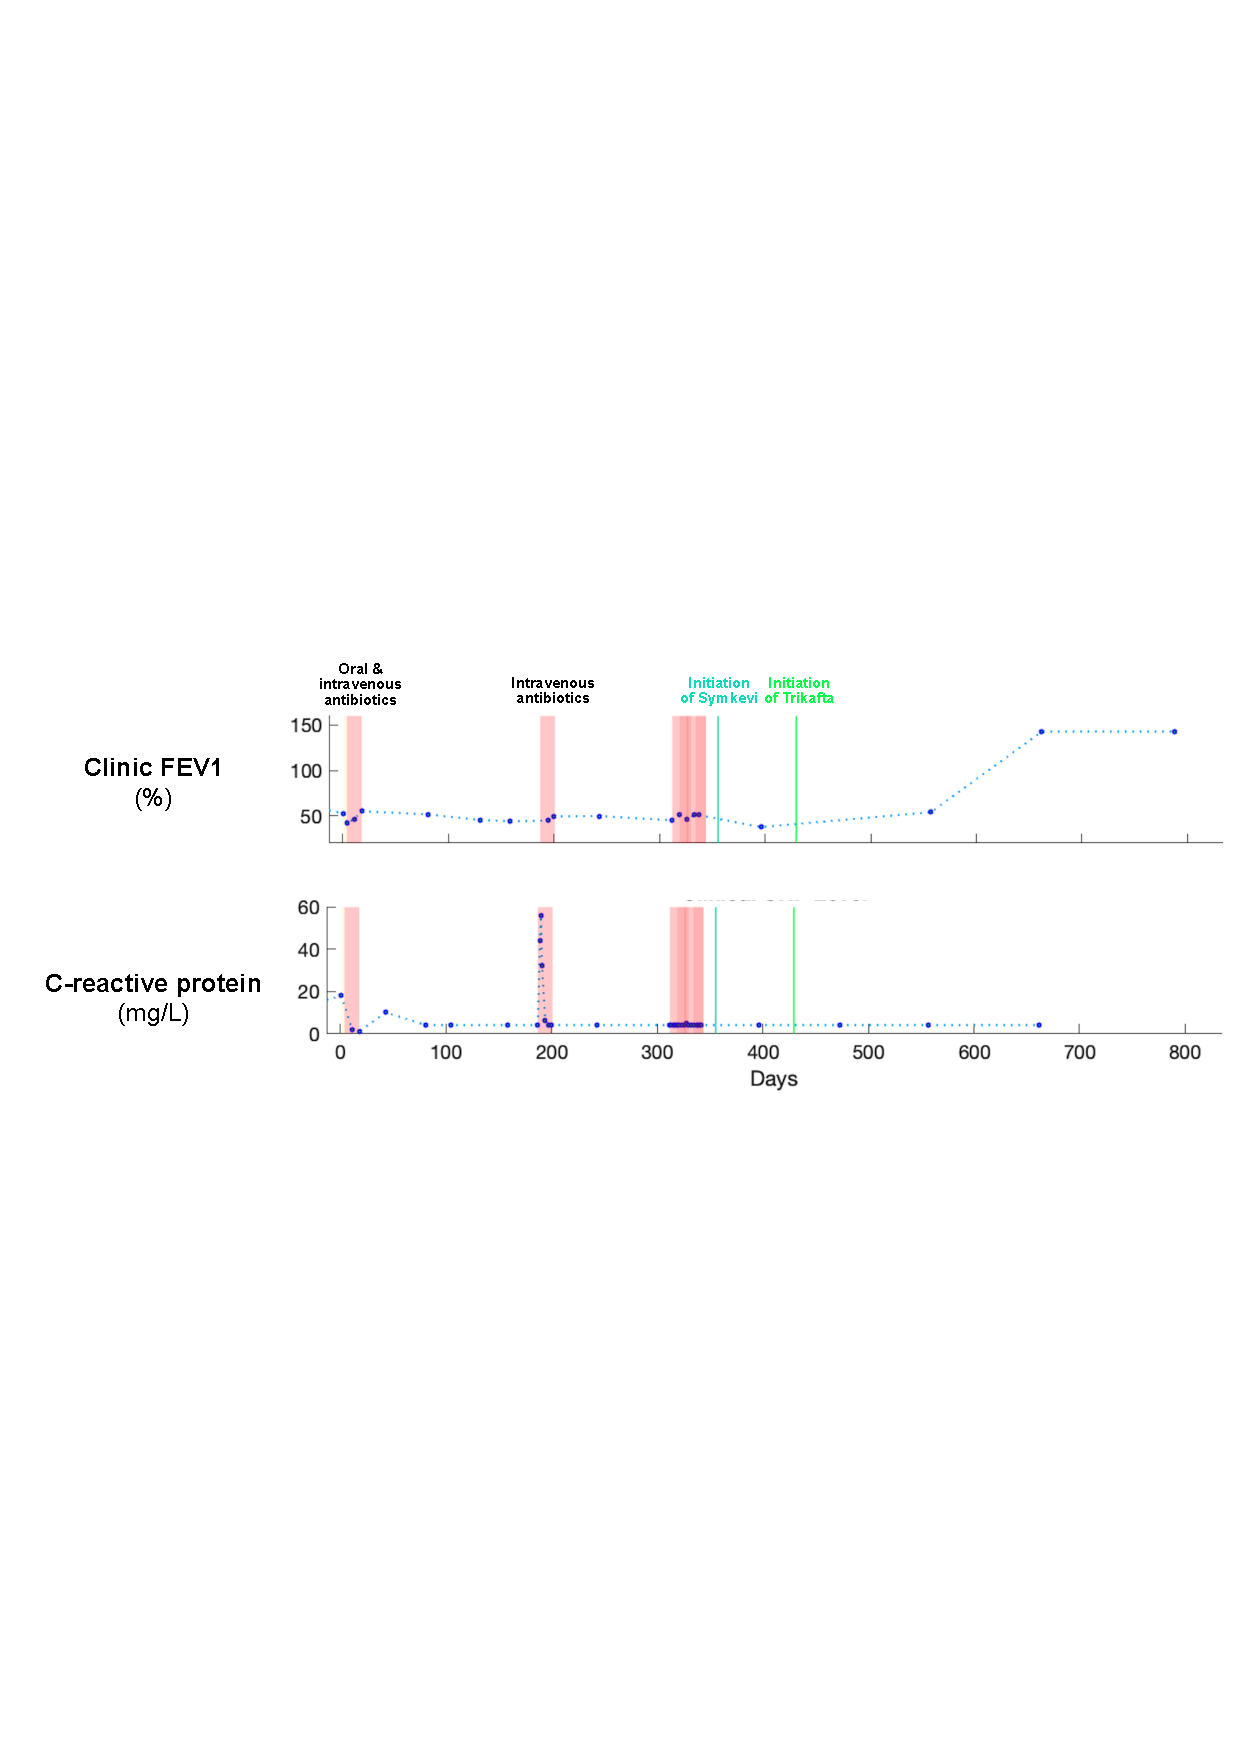
\includegraphics[width=96mm]{images/clinicdata.pdf}
    \label{fig:clinic}
    \end{figure}
    
    \begin{figure}[!h]
    \caption{Home measurements data, with patient measures' mean and standard deviations}
    \centering
    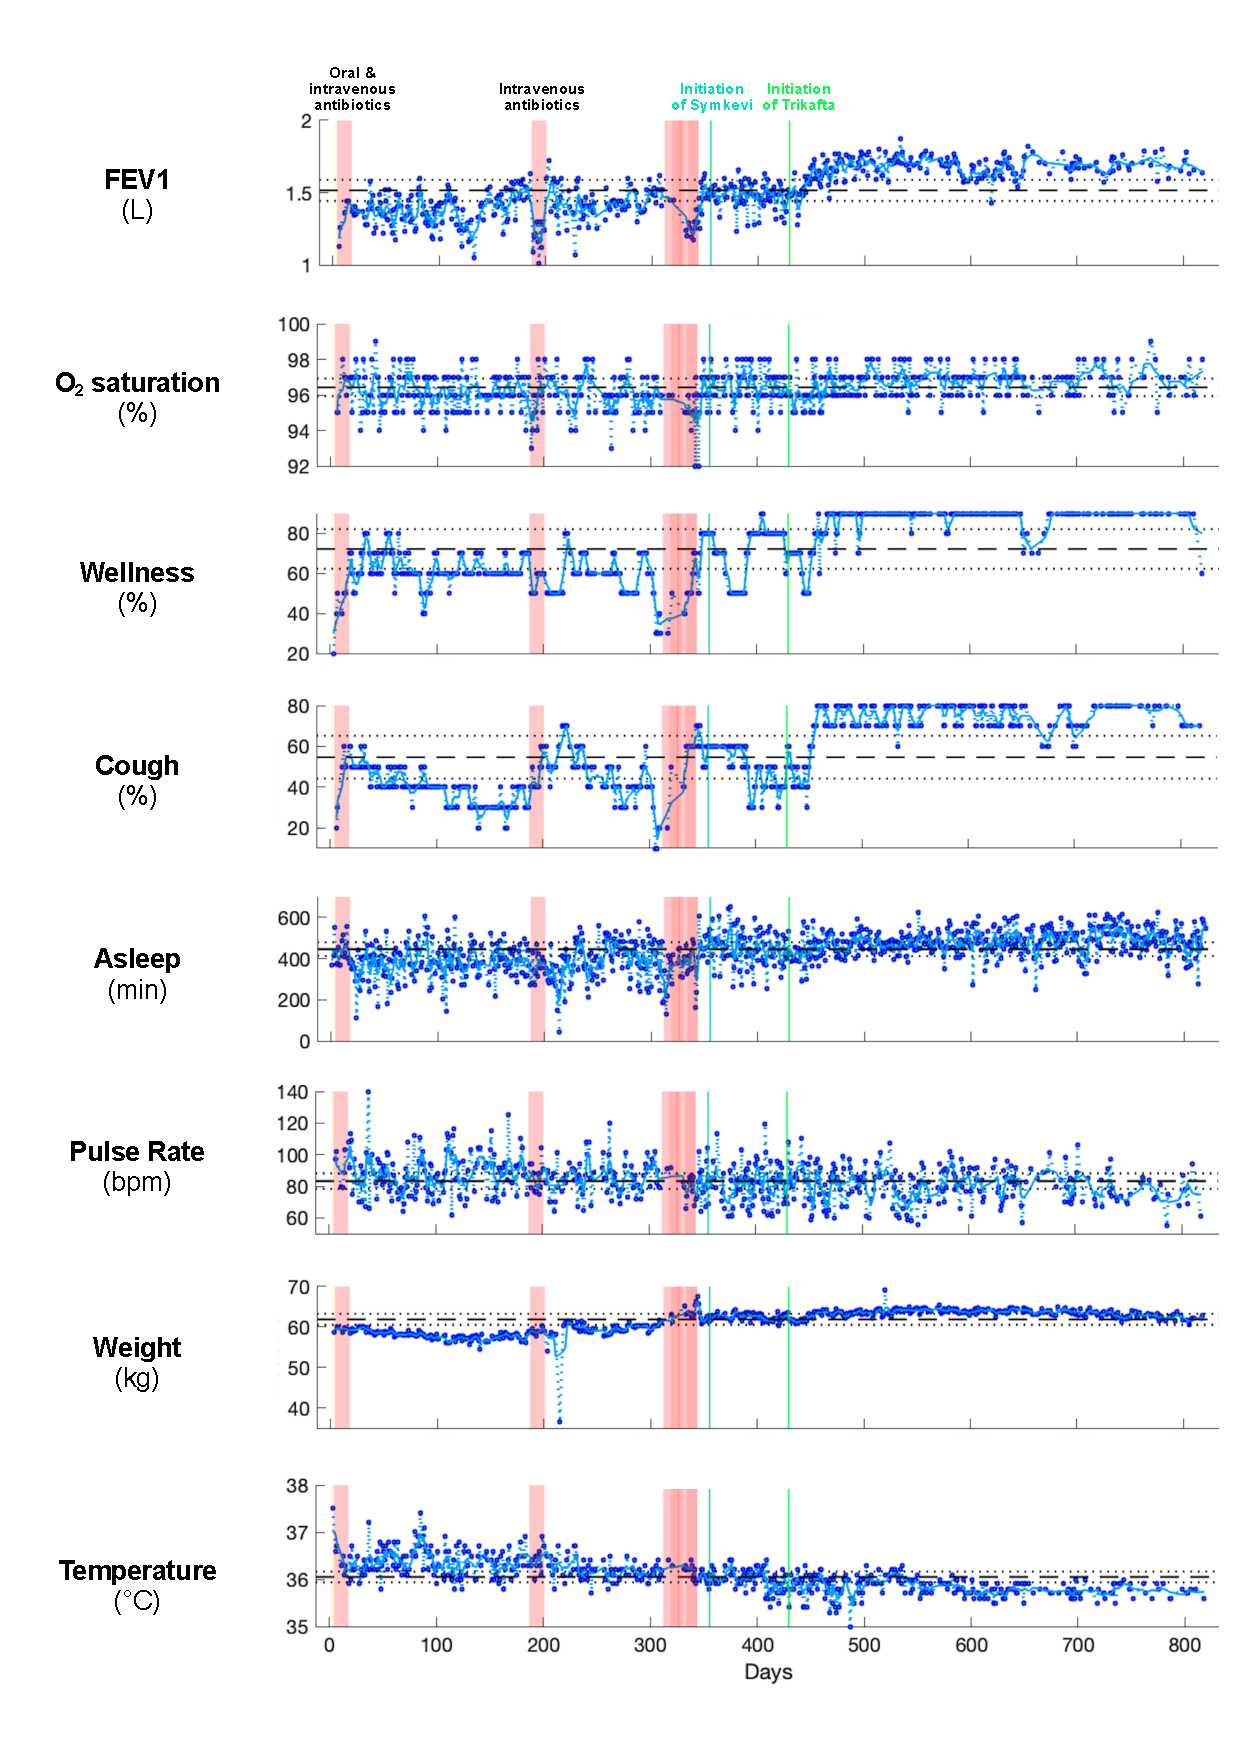
\includegraphics[width=96mm]{images/homedata.pdf}
    \label{fig:home}
    \end{figure}

\chapter{Data quality check}
A rigorous process of data quality assurance was conducted on both the clinical meta-data and the home measurement data. A summary of the specific cases and related actions is detailed in Figure \ref{fig:dataqualitycheck}.

For the clinical data, potentially anomalous values for FEV1, age, weight, height, CRP were identified, as well as inconsistencies between the different types of meta-data – for example a hospital admission without an antibiotic treatment. Whilst not definitively highlighting a data problem, such items were sent back to each of the centres for review and any necessary corrections were applied to the data set.

For the home measurement data, a similar process to identify potentially anomalous values was applied, resulting in a small number of suspect data points being excluded. In addition, data uploads before and after midnight were analysed to ensure they were applied to the correct date. Finally, there were a number of data records with more than one recording for a given measure on a given day – which could have indicated a problem with an automated upload to the servers, or an intentional correction to a previously entered number, or genuinely taking multiple readings per day. A detailed analysis was performed, and corrective actions were taken where possible.

    \begin{figure}[!h]
    \caption{Data quality check and actions performed}
    \centering
    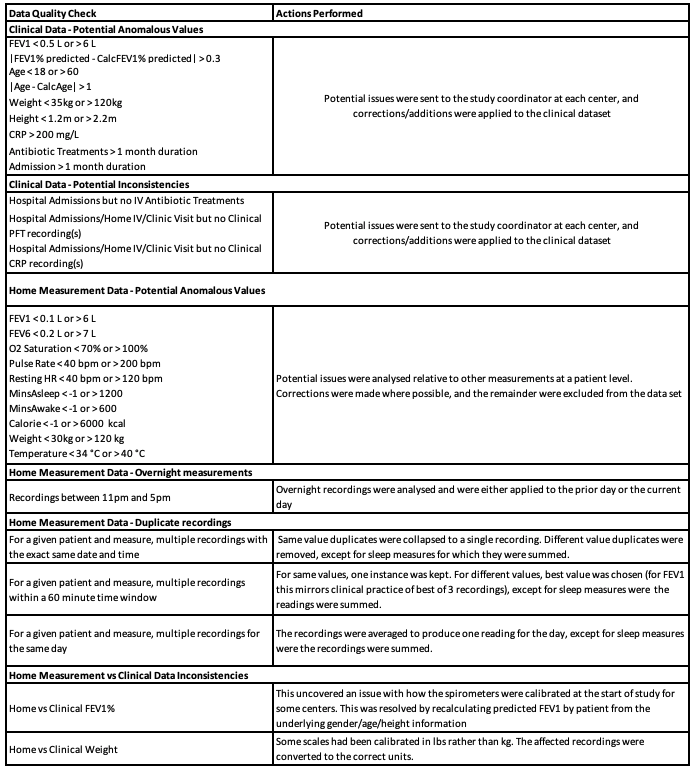
\includegraphics[width=150mm]{images/dataqualitycheck.png}
    \label{fig:dataqualitycheck}
    \end{figure}

\chapter{Examples of three participants interventions profiles} \label{sec:appendixint}
Figures \ref{fig:intrfull}, \ref{fig:intrivpbo} and \ref{fig:intrdecline} respectively show a full recovery from 14 days IV treatment, a successful recovery from 20 days of IV treatment preceded by oral treatment (IVPBO), an unsuccessful recovery characterised by a continuous decline despite treatment. The data records used by the probabilistic inference algorithm ranges from day 0 to day 20 from this graph. The stable baseline is defined as the mean of the upper 75\% of measurements from 35 to 25 days prior to treatment. Note that 1) on the profiles, the temperature, and pulse rate are inverted, and 2) an increase in wellness and cough (displayed in percentage) indicate a diminution of wellness, respectively cough.
    
    \begin{figure}[!h]
    \caption{Successful recovery (back to stable baseline and stabilisation for most measures) delayed due to stacked antibiotics: IV preceded by oral (IVPBO)}
    \centering
    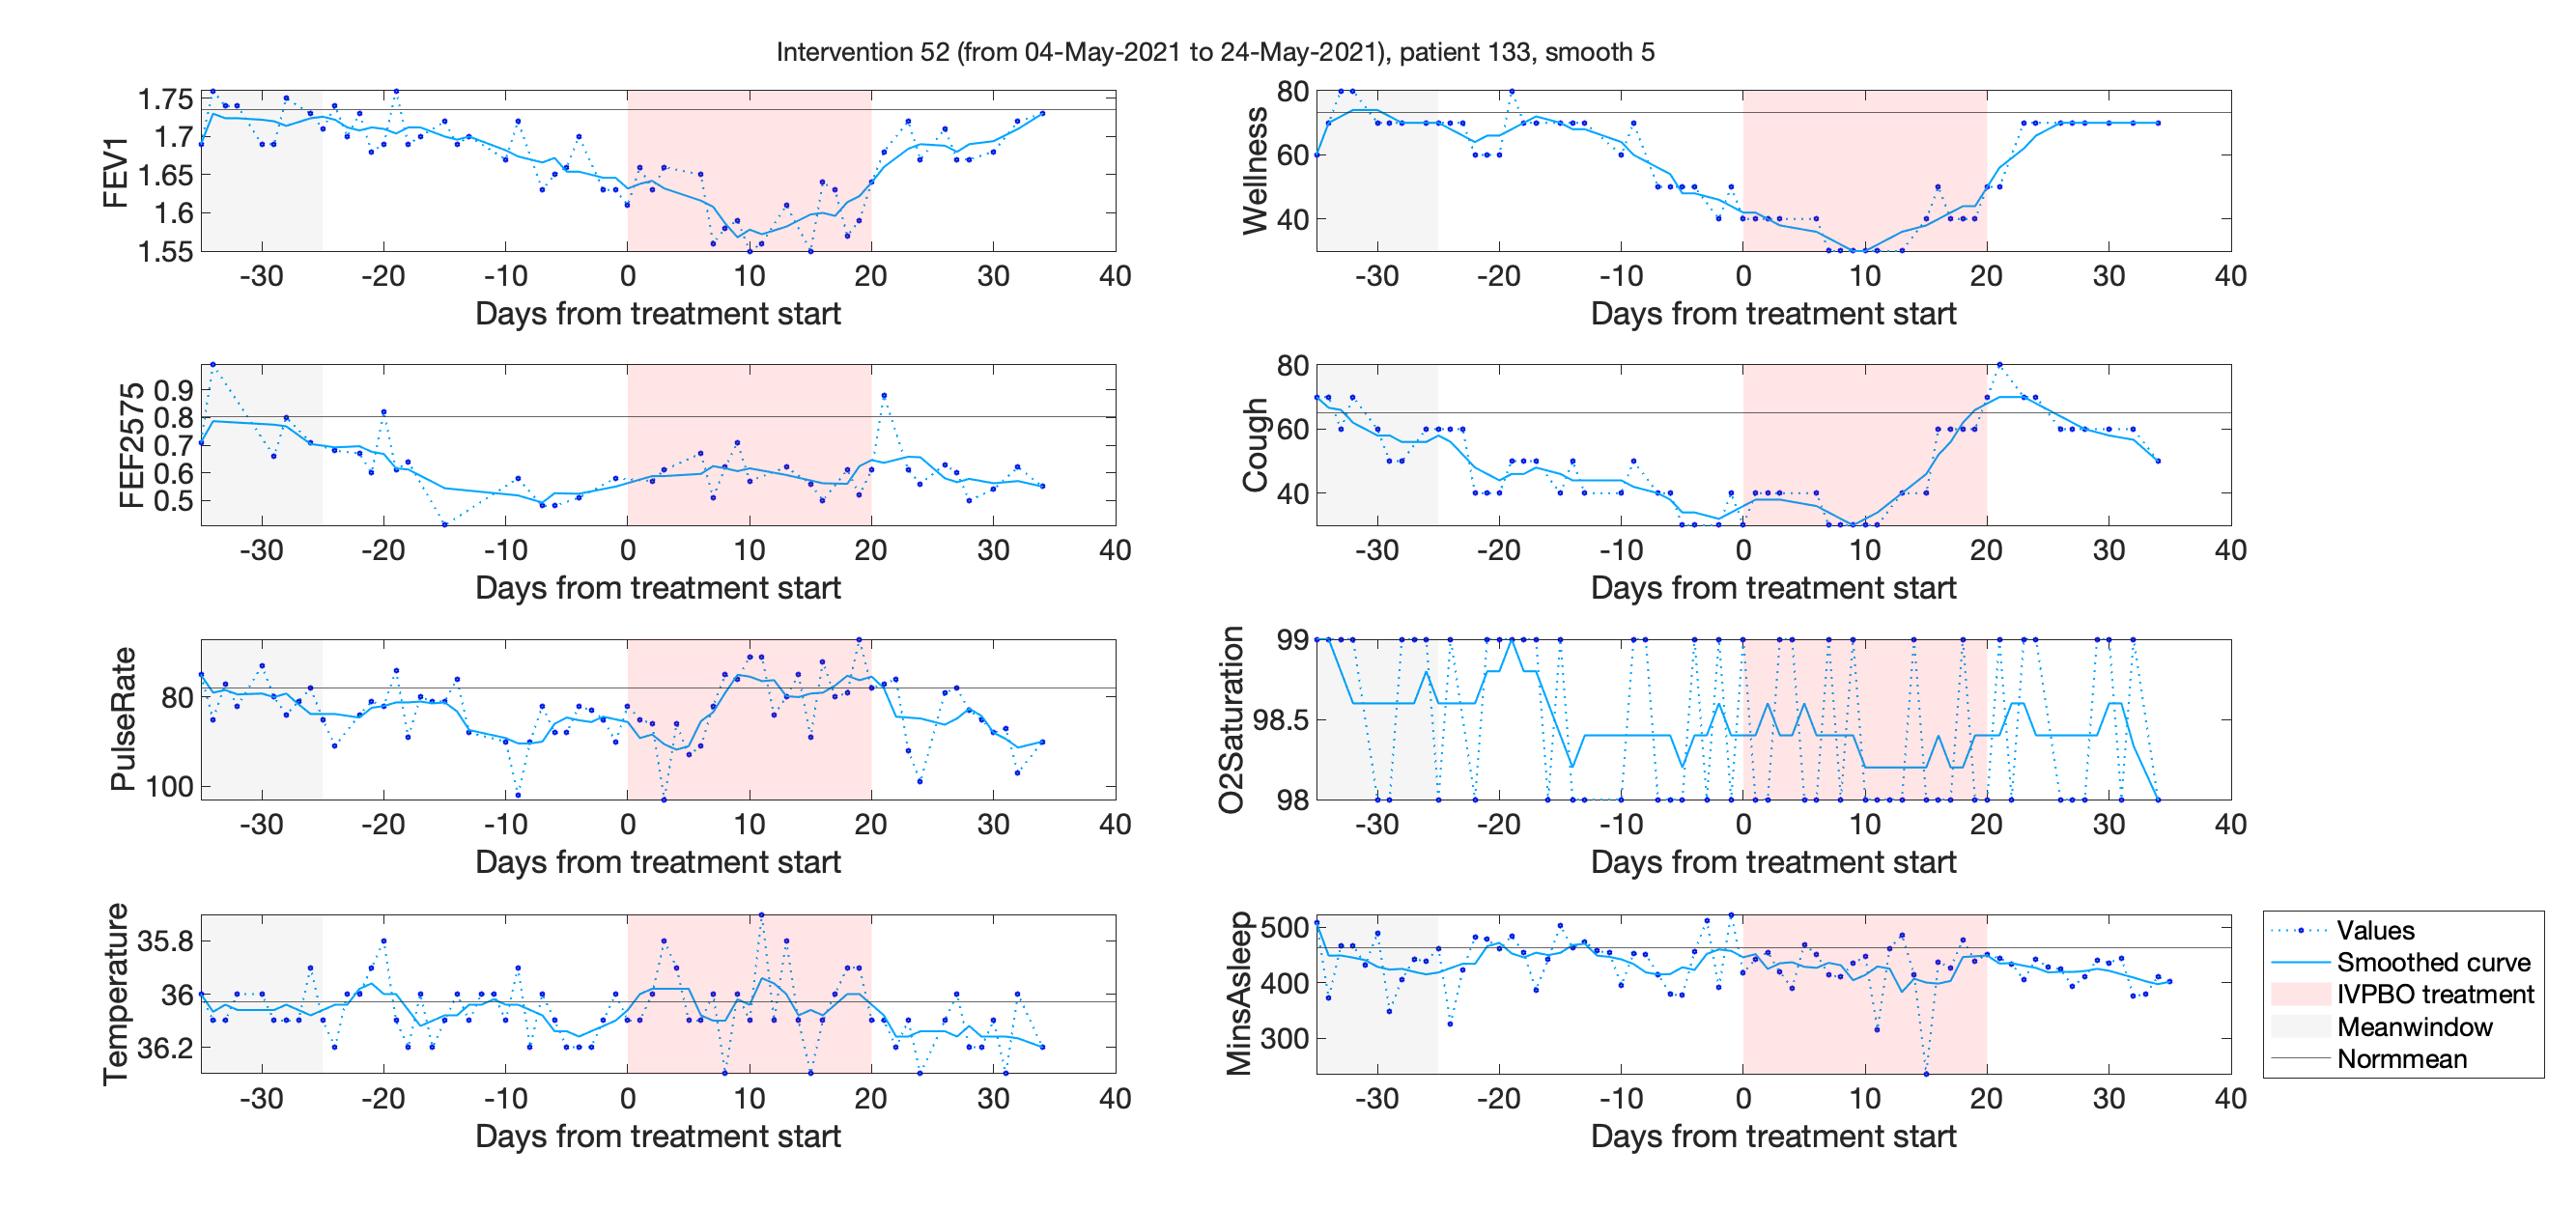
\includegraphics[width=150mm]{images/Intervention52_ID133.png}
    \label{fig:intrivpbo}
    \end{figure}
    
    \begin{figure}[!h]
    \caption{Full recovery (back to stable baseline with overshoot) followed by decline from IV treatment}
    \centering
    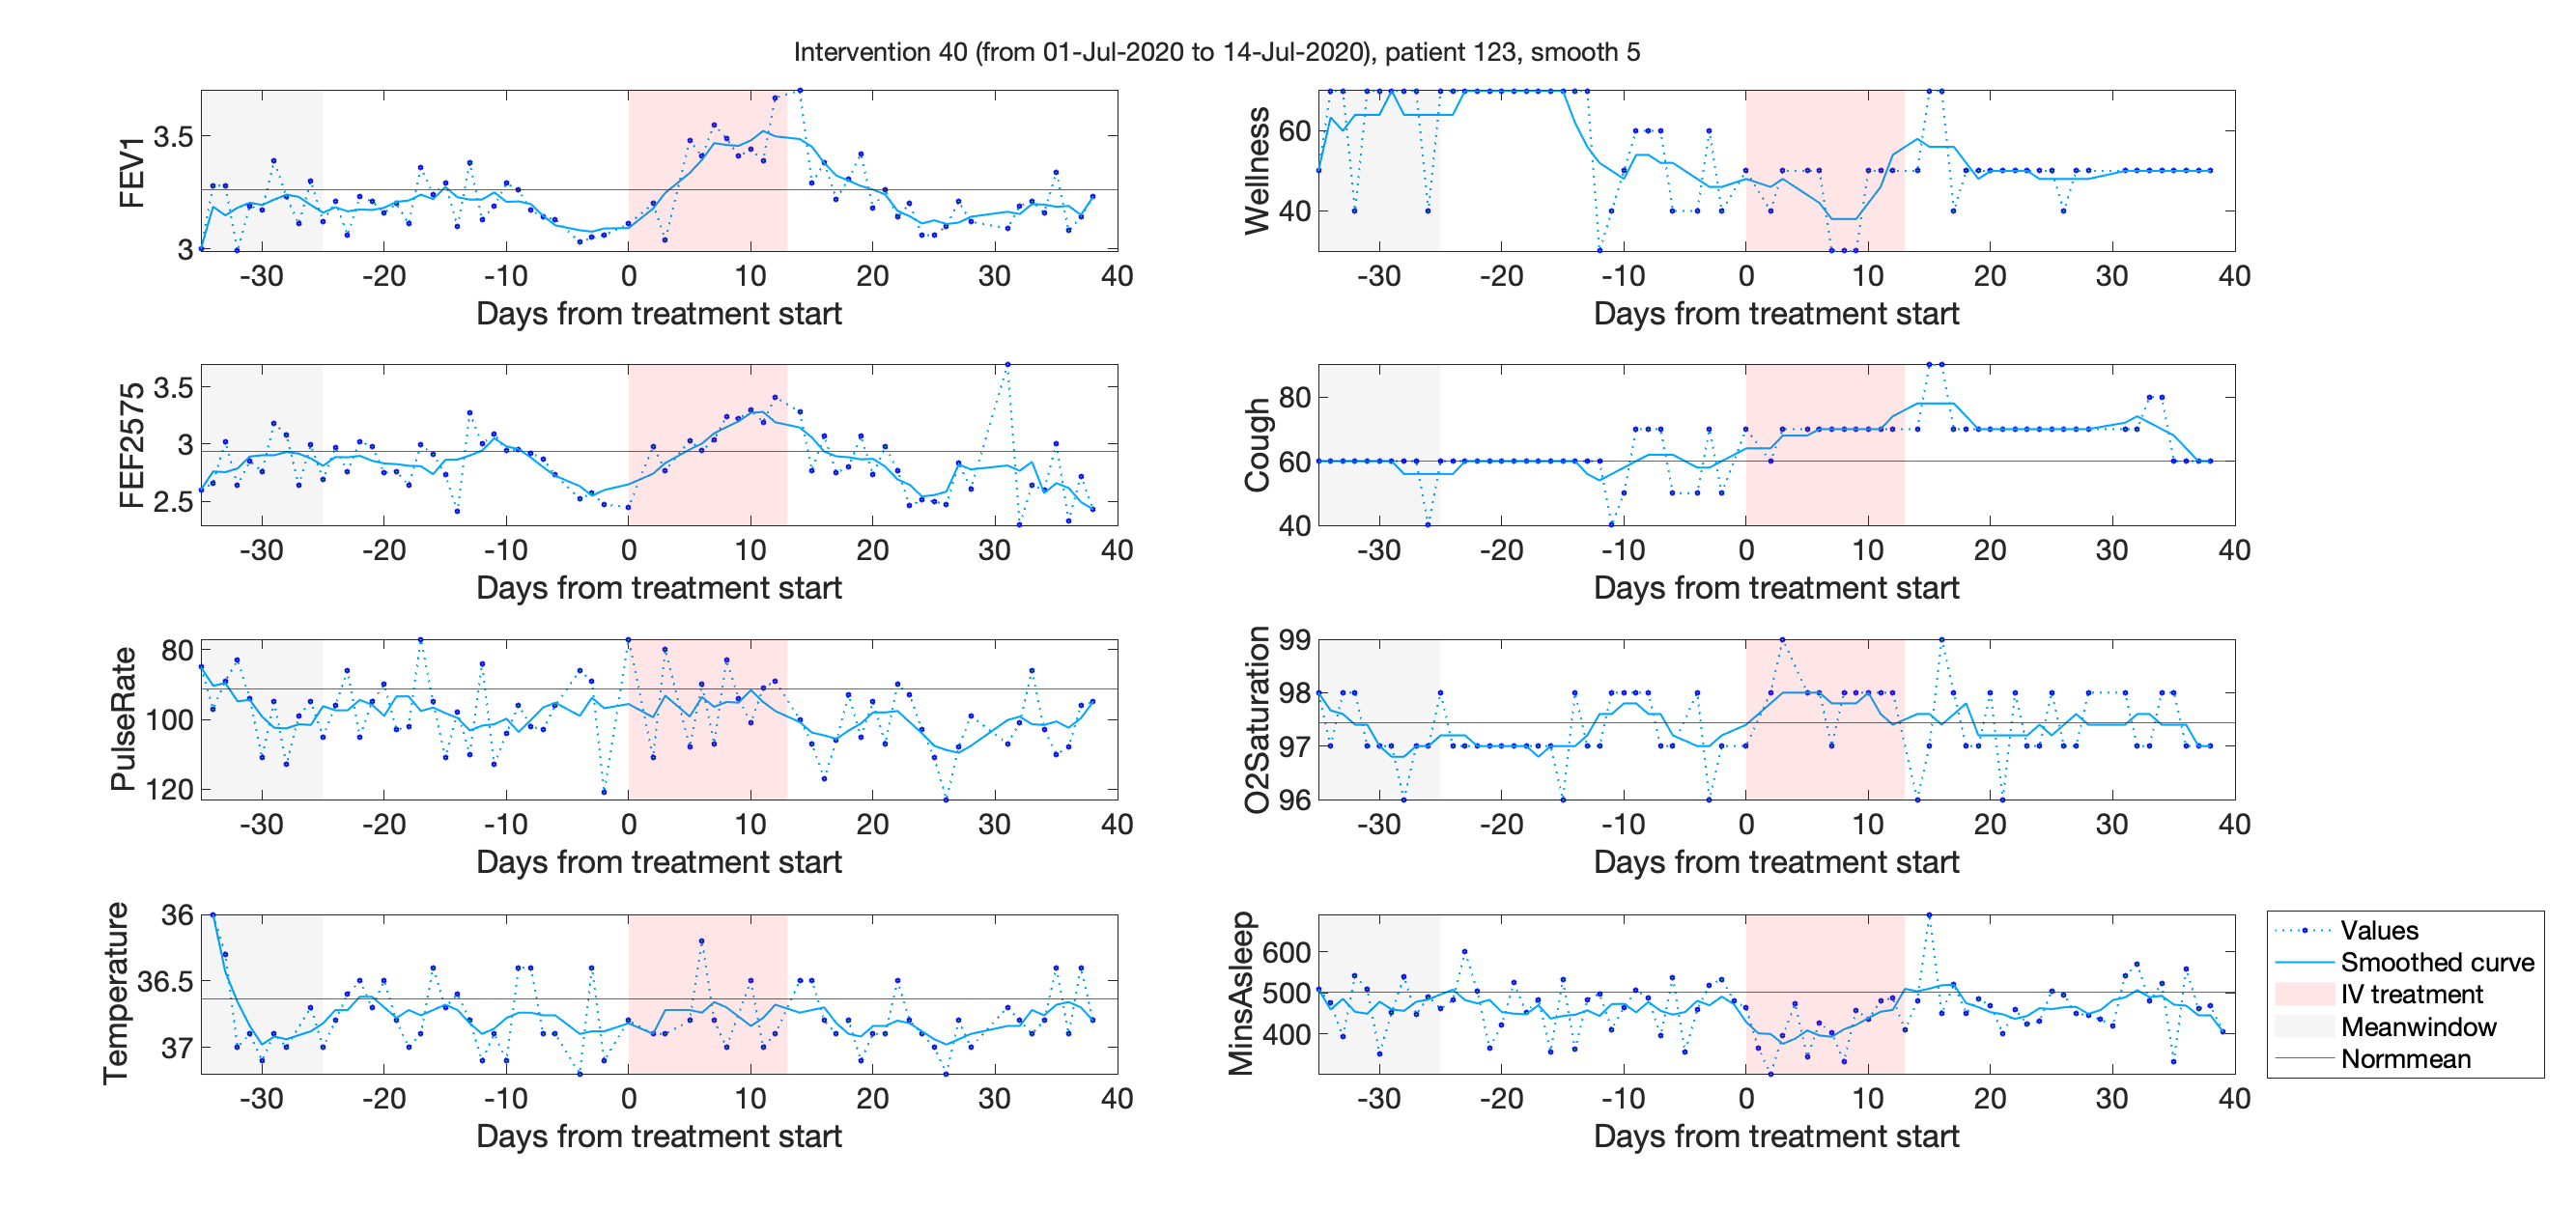
\includegraphics[width=150mm]{images/Intervention40_ID123.png}
    \label{fig:intrfull}
    \end{figure}
    
    \begin{figure}[!h]
    \caption{Continuous decline despite oral antibiotic treatment}
    \centering
    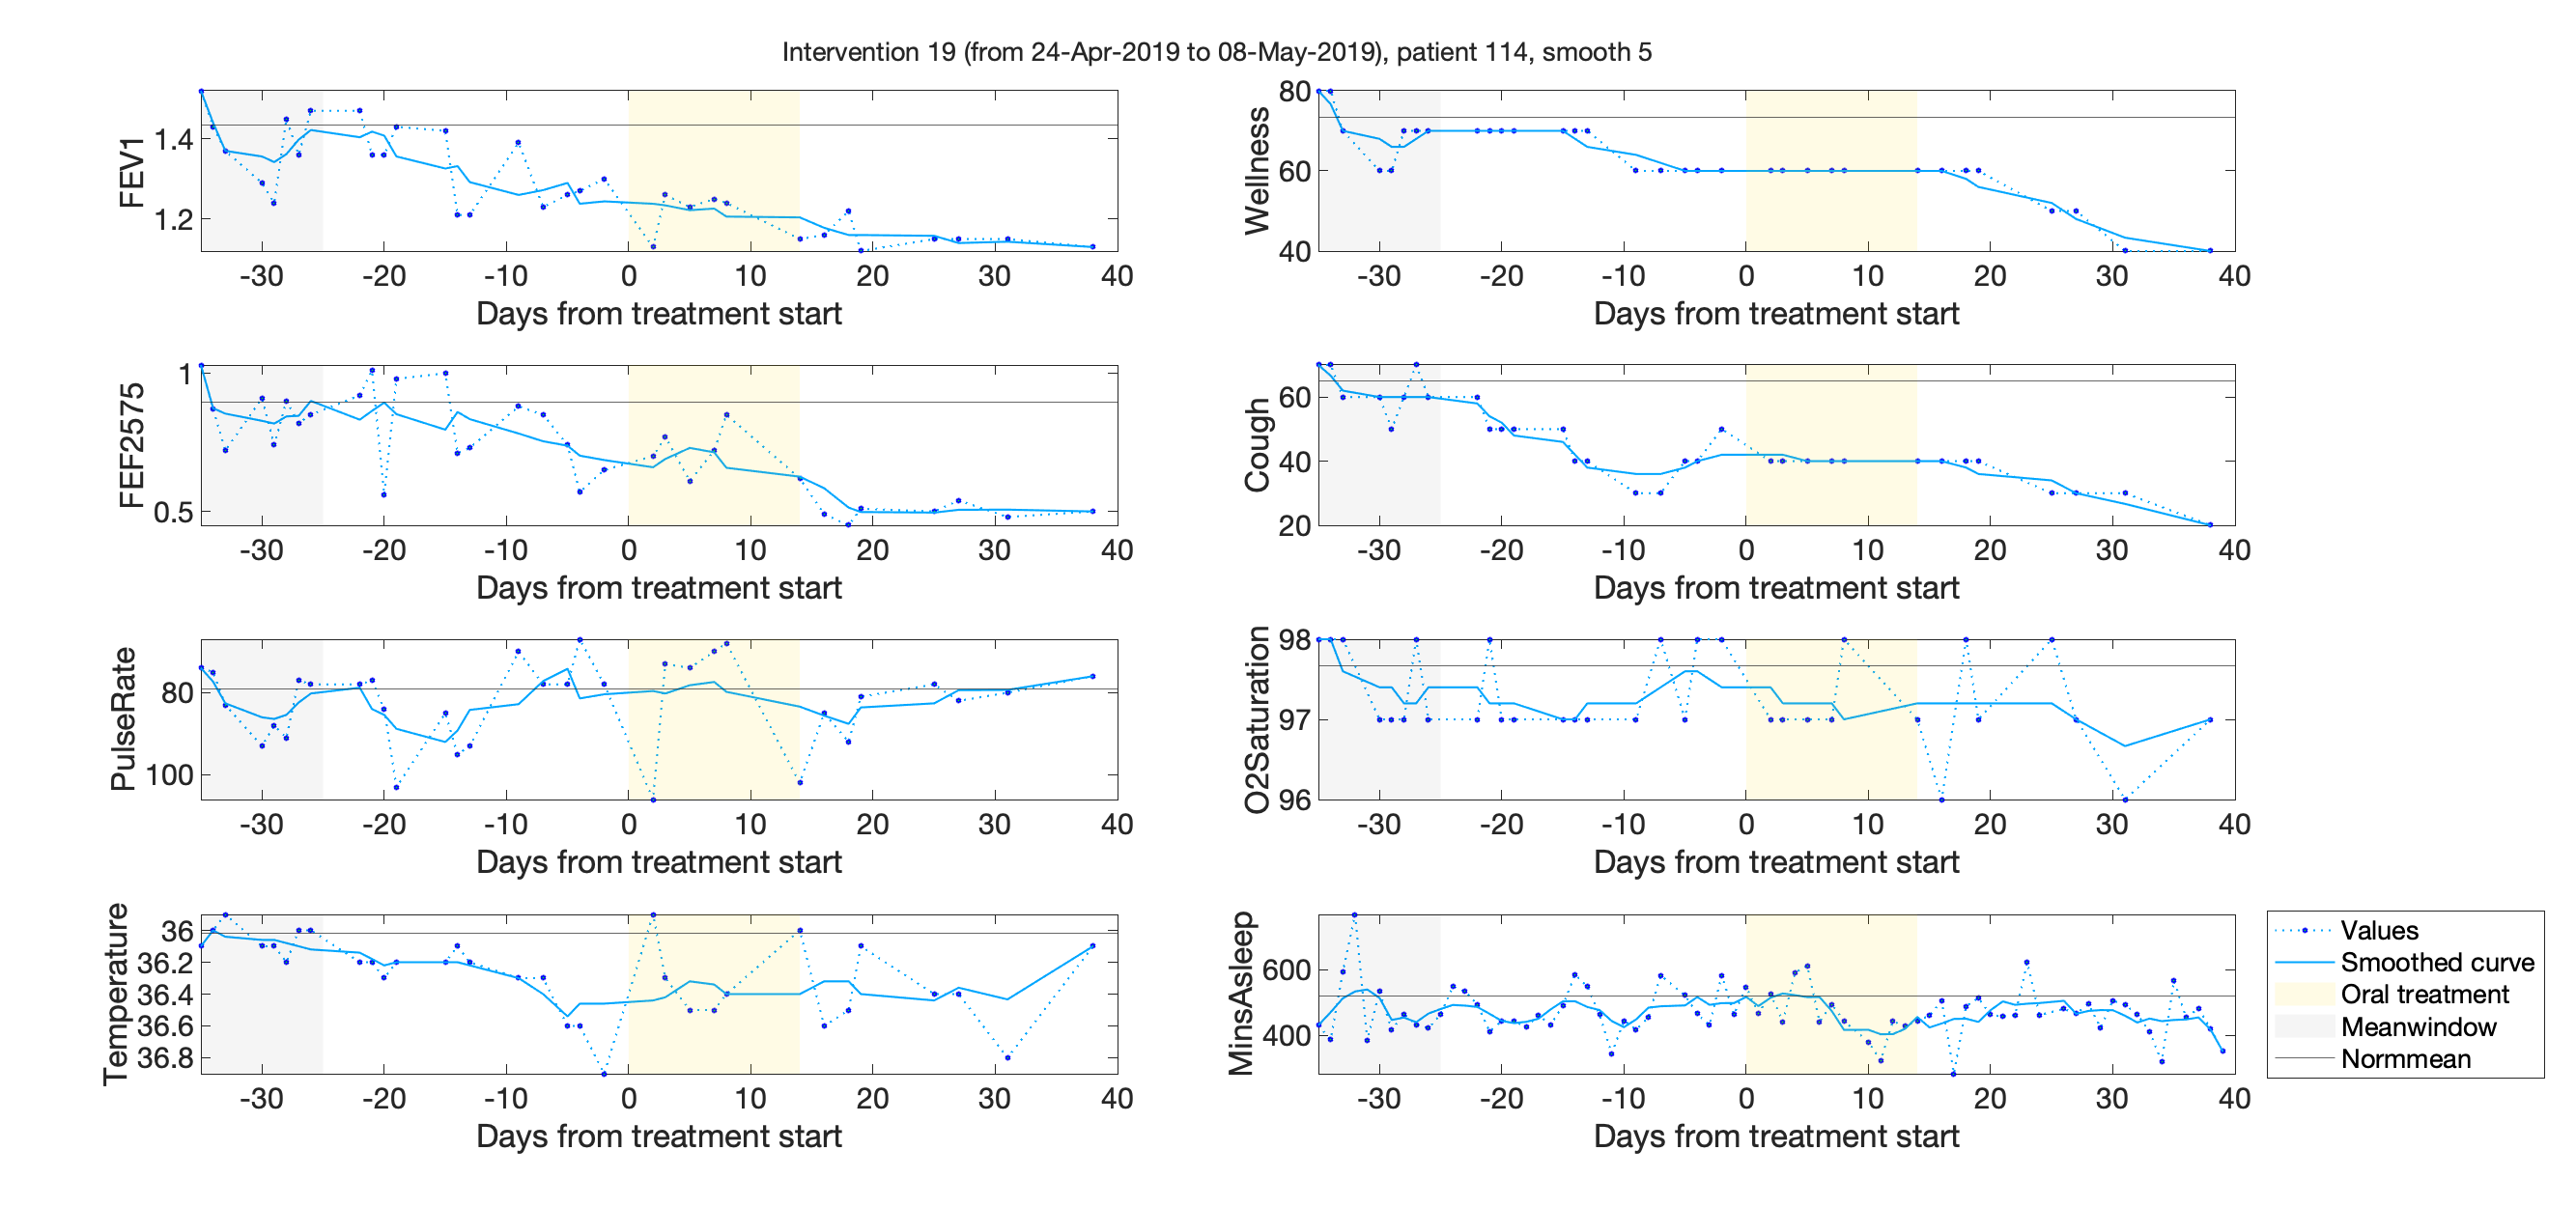
\includegraphics[width=150mm]{images/Intervention19_ID114.png}
    \label{fig:intrdecline}
    \end{figure}
    



    
\end{appendices}